\documentclass{article}
\usepackage{graphicx}
\usepackage{subcaption}  % Add this in your preamble
\usepackage[margin=1in]{geometry}
\usepackage[backend=bibtex,style=authoryear]{biblatex} % or 'style=numeric'
\addbibresource{research_proposal.bib}  % filename of .bib file
\usepackage{hyperref}

% set graphics path
\graphicspath{{/Users/danpost/housing_project/output/planning_commission_project/graphics/}}

\title{The Market for Housing Regulation - Application to San Francisco}
\author{Daniel Posthumus}

\begin{document}

\maketitle

\tableofcontents

\clearpage

\section{Introduction}

In housing markets across the United States, there are two markets: the economic and the political. These two markets interact in endogenous ways, as outcomes in one engage in a cycle of causality with outcomes in the other. These interactions are economic, political, and sociological in nature because of the multi-dimensional utility of housing, as consumption of housing entails benefits far exceeding the material. Housing affects educational opportunities, feelings of personal safety, political power, ease of commuting, access to amenities, among other areas of well-being. In this way, \textit{consumption} of housing is complex and multi-dimensional; so is organizing the market for housing, which is done through intensely political means in the market for regulation. At the heart of these interactions, then, is the political economy of housing regulation -- in particular, how these regulations come into being and how they are implemented. Here I study these two aspects of housing regulation -- focusing on the first qualitatively and the second quantitatively.

I argue that the political economy of housing remains deeply under-studied, for two primary reasons. The first is that the outcomes in either of the two housing markets -- political or economic -- are endogenous to the other. This is particularly true for the market for regulation; to what extent are political rather than economic forces driving the politics of housing regulation? Because political forces alter local economies in ways more varied than just housing, tracing changes in the economic state of housing to politics, and vice-versa, is difficult. This leads me to the second reason this political economy is under-studied. One way to counter this endogeneity is to avoid cross-sectional analysis and engage in panel analysis. This allows the researcher greater control in accounting for history, culture, social dynamics, and other observables. Engaging in panel analysis, however, requires a panel dataset -- and no comprehensive panel dataset of housing regulations in the United States exists. Below I discuss the two existing datasets of housing regulations, and why they fail to satisfy the needs of any model aiming to explain outcomes in the market for regulation.

Accordingly, I propose another type of dataset and apply this framework to building a dataset of regulation using meeting minutes dating back to 1998 for San Francisco's (SF) Planning Commission. Here, I focus on introducing this dataset and establishing descriptive facts about the going ons of the San Francisco Planning Commission. Finally, I conclude this work with the outline of a broader and more ambitious model of housing in the Bay Area, which would require the application of this approach to the differing regulatory polities within the Bay.

\section{Motivation}

Housing has taken center stage in discussion of US policies and governance. Two clear stories emerge with respect to affordability. 

First, one story is that the scope of the housing crisis at the center of the endlessly-discussed \textit{Abundance} agenda is rather narrow. 

Second, if we zoom in on the centers of productivity in the economic geography of the United States, a much more drastic and urgent picture emerges. 

Then, if we accept that many metropolitan areas with very high productivity are building less housing than they should be, let's say that a community does \textit{not} want more housing. Then, there are multiple ways for communities to engage in the market for regulation within communities.  One way is to use political power to alter the rules/market organization of the housing market by supporting certain zoning reforms or policies that restrict the housing supply. Though not strictly related to the housing supply, the recent closing of the Great Highway in San Francisco through the successful passage of Proposition K is an excellent example.

Proposition K, the subject of which is "Permanently Closing the Upper Great Highway to Private Vehicles to Establish a Public Open Recreation Space' \footnote{See \href{https://voterguide.sfelections.org/local-ballot-measures/proposition-k}{this voter guide} from the San Francisco City Government. The exact question on the ballot was ``Shall the City use the Upper Great Highway as public open recreation space, permanently closing it to private motor vehicles seven days a week, with limited exceptions?"} was put on the ballot by elected supervisors of the San Francisco Board of Supervisors. It was then put to the residents of San Francisco on a simple yes/no vote, requiring 50\% + 1 to pass. It did pass, with 54.73\% vote of the vote; for context, the proposition received more affirmative votes than either Daniel Lurie or London Breed (the two leading mayoral candidates) did in the 14th and final round of Ranked-Choice Voting. It was clear during, and in the wake, of campaigning over the measure that this was a regulation subject to the usual YIMBY (`Yes In My Backyard') and NIMBY ('No In My Backyard'). Below as Figure \ref{fig:prop_k_motivation} I've included an exemplary instance of paid argumentation \textit{against} the measure which makes this link clear; remember that the measure itself contains no explicit mention of housing.

\begin{figure}[hbt]
\centering
\begin{subfigure}[b]{0.8\textwidth}
	\centering
	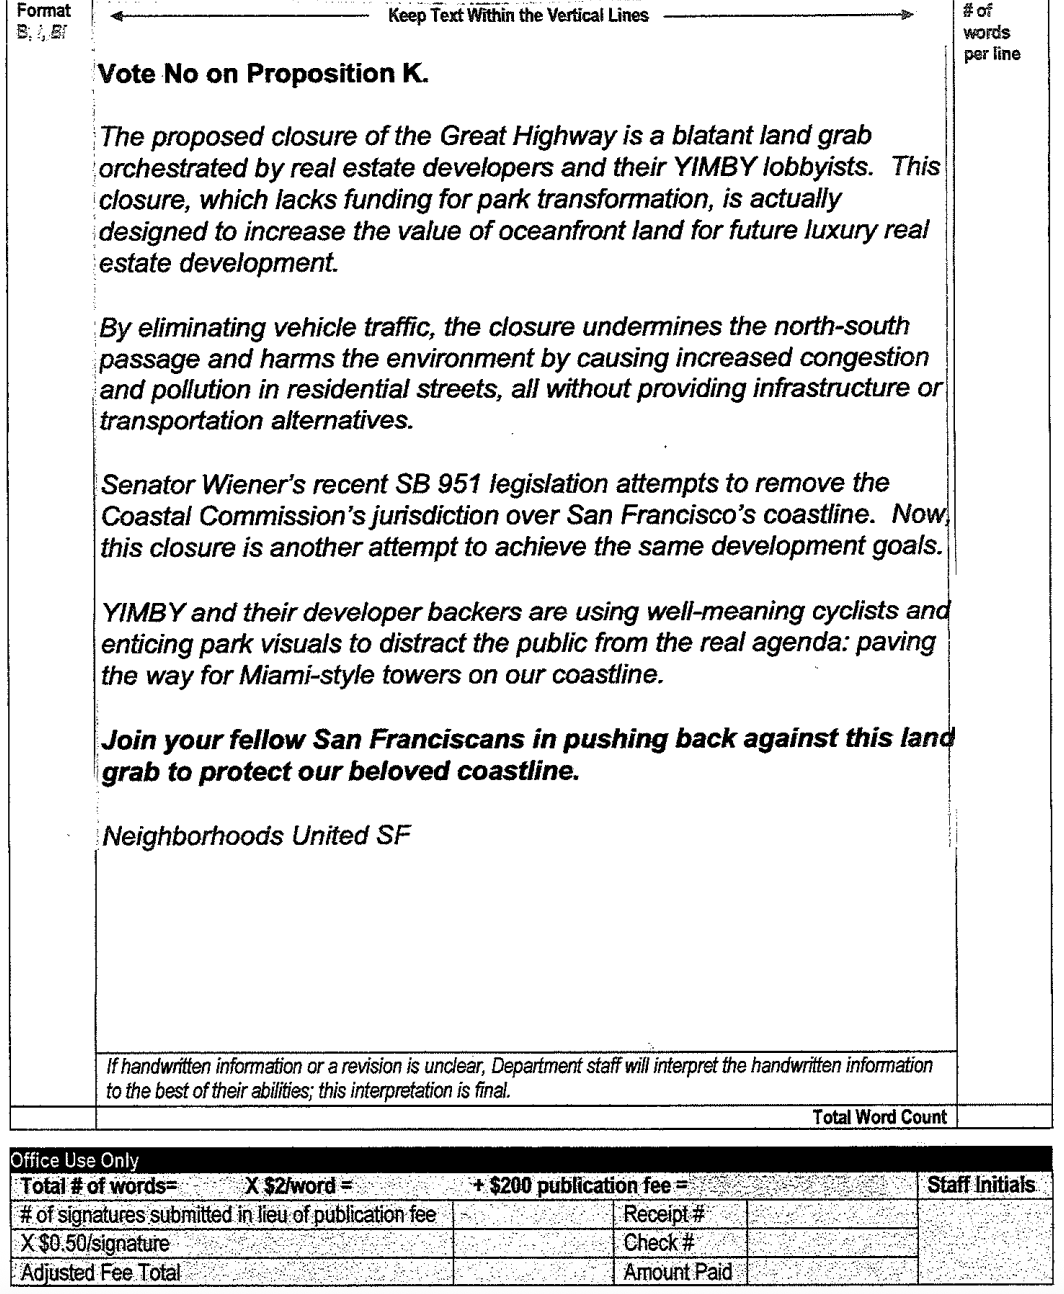
\includegraphics[width=\textwidth]{prop_k_statement_1.png}
\end{subfigure}
\caption{Proposition K in San Francisco Was Hotly Contested by Active Forces in the Market For Regulations}
\label{fig:prop_k_motivation}
\end{figure}

Another way is to use political power to support candidates for local government who don't \textit{alter}  rules or regulations, which may be politically expensive, but instead operate government in such a way that restricts construction. This can be through organs of local government. Perhaps members of the community can mobilize and forcefully argue their case in public hearings or meetings of the Planning Commission, lobbying members to not approve either the issuance of permitting or specific instances of rezoning. Or perhaps members of a community could push their elected representatives to fight for a `historic designation' for their community, which may halt construction and development regardless of zoning laws. For example, in Figure \ref{fig:historic_prev_motivation} we can see concerns emerge that neighborhoods are adopting this as a strategy to avoid development.\footnote{See \parencite{Li2025} and \parencite{Appelbaum2023}.}

\begin{figure}[hbt]
\centering

\begin{subfigure}[b]{0.8\textwidth}
    \centering
    \includegraphics[width=\textwidth]{motivation_screenshot_1.png}
\end{subfigure}

\begin{subfigure}[b]{0.8\textwidth}
    \centering
    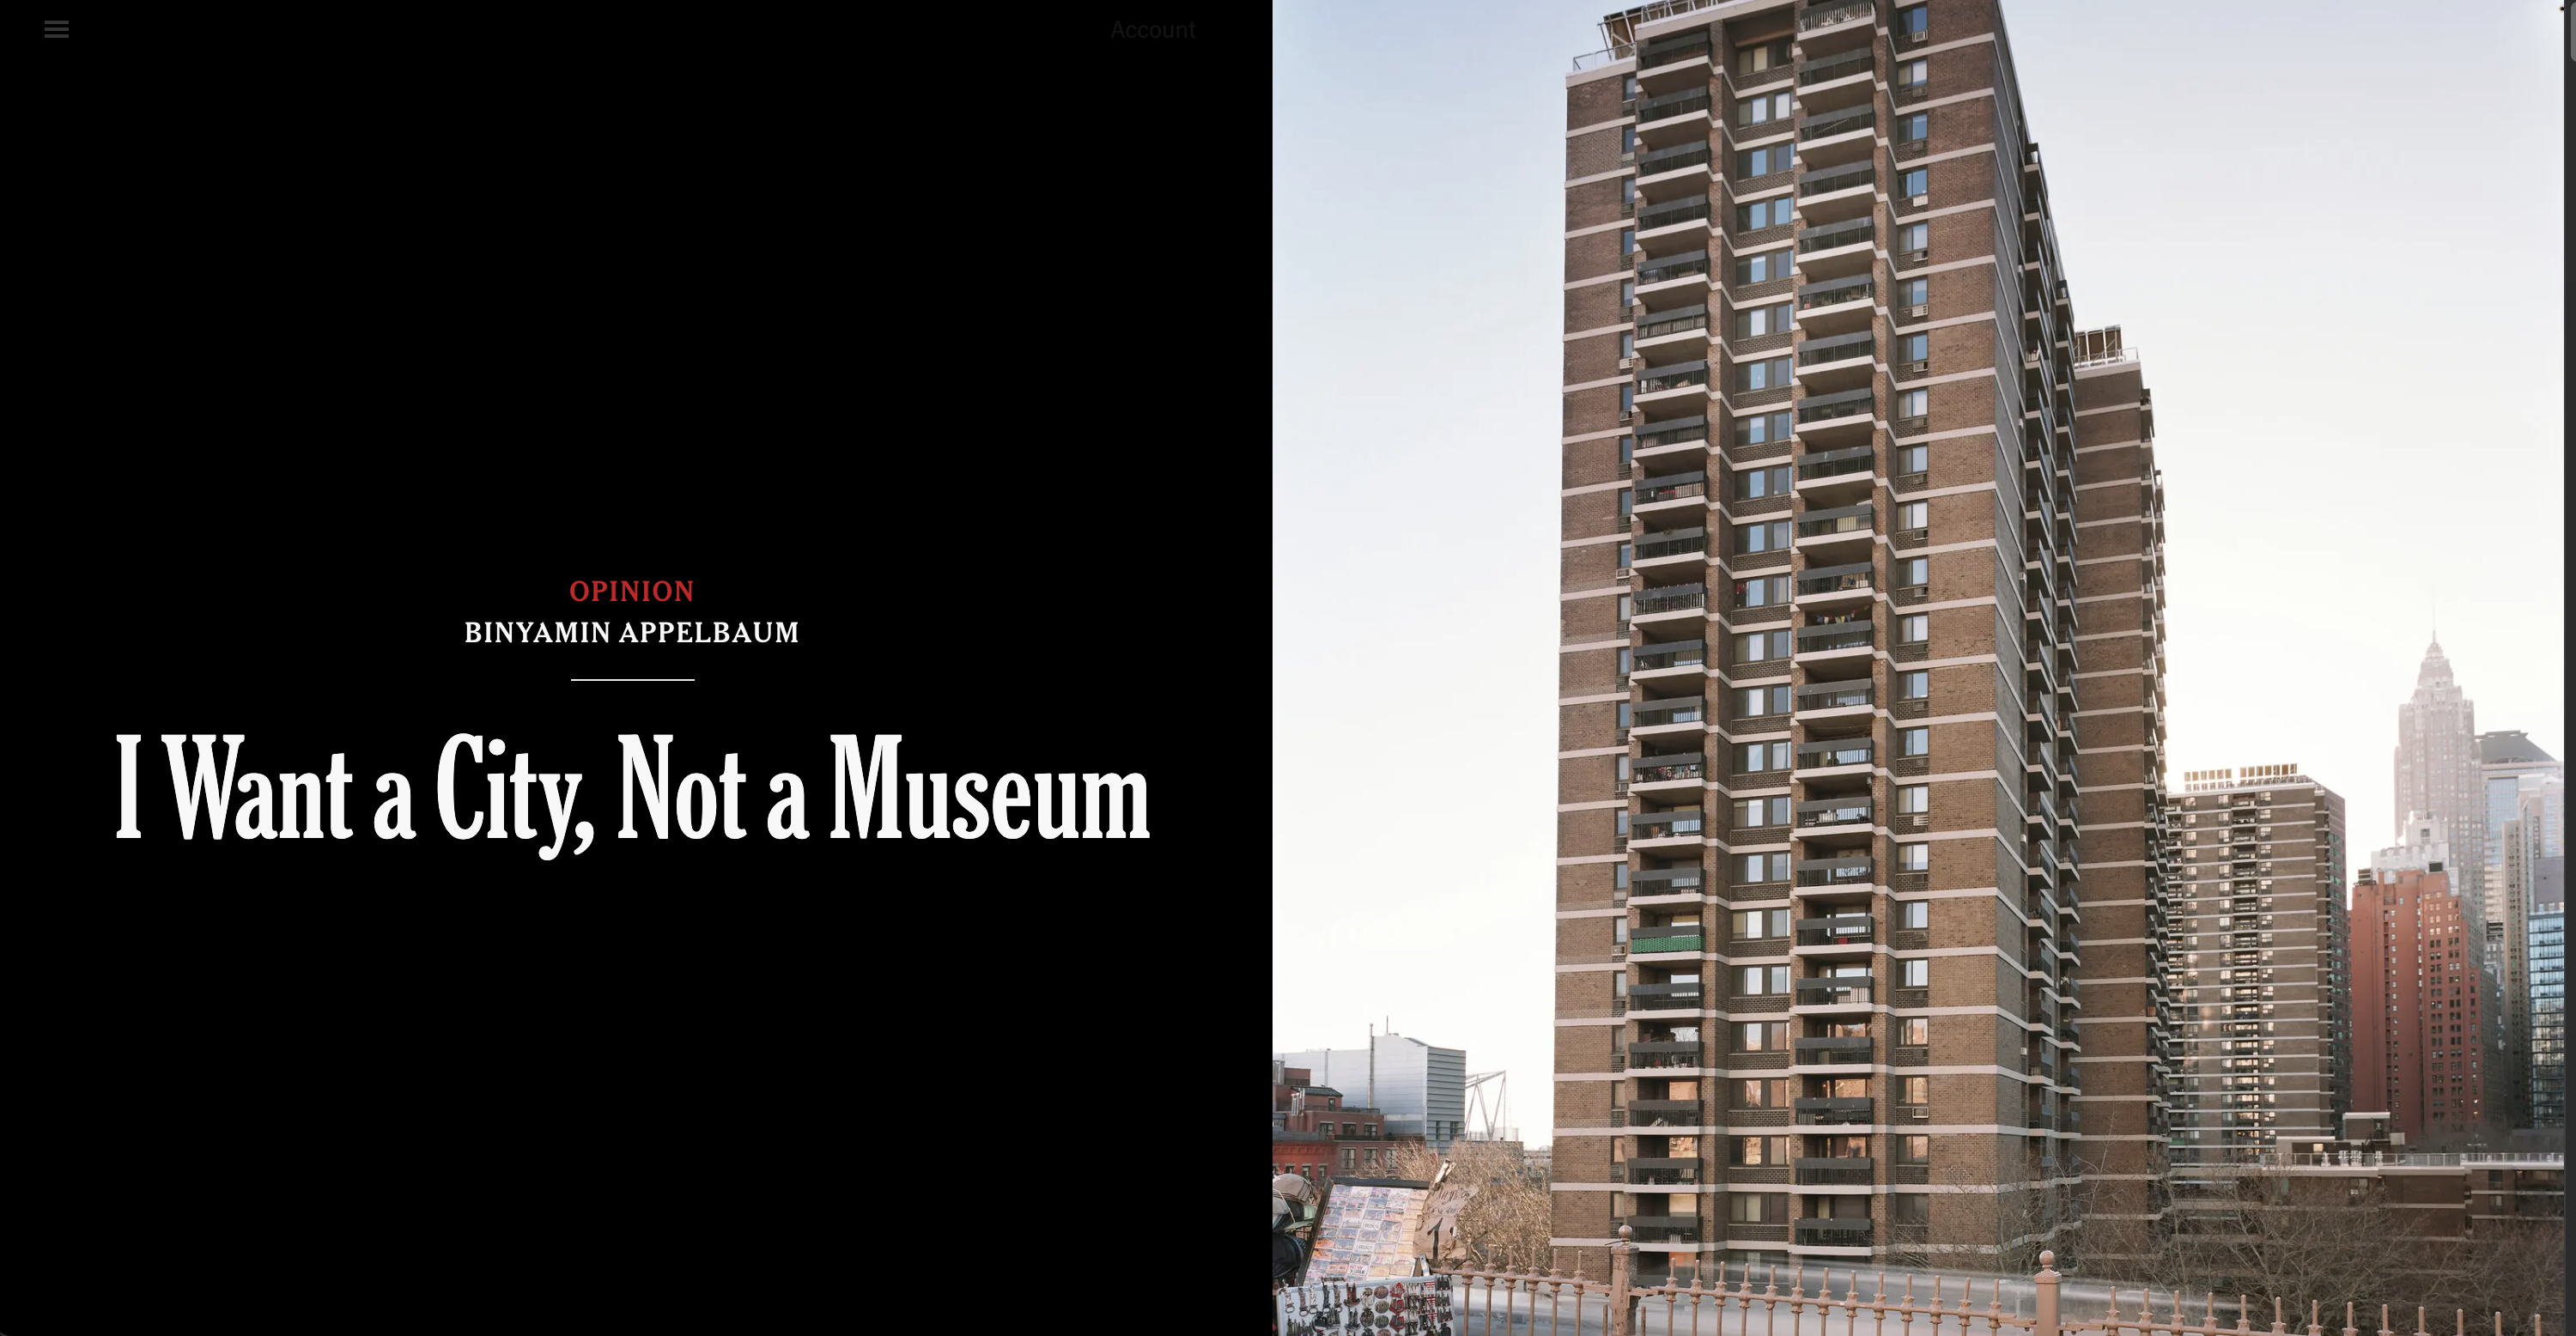
\includegraphics[width=\textwidth]{motivation_screenshot_2.png}
\end{subfigure}
\caption{There is an emergent awareness in how markets for regulation are interacting with markets for housing.}
\label{fig:historic_prev_motivation}
\end{figure}

\section{Literature Review}



\subsection{Data Constraints}



\section{History of Planning and Housing Regulation in San Francisco}



\subsection{Structure of Housing Regulation in San Francisco City Government}




\section{A Simple Theoretical Model of the Market for Housing Regulation in California}



\section{Applying Large Language Model (LLM) to the San Francisco Planning Commission Minutes}



\section{Results from San Francisco Planning Commission Minutes}



\section{Modeling Market for Regulation and Housing in the Bay Area - Next Steps}


\clearpage

\printbibliography


\end{document}